
\documentclass[]{spie}

% Package imports go here.
\renewcommand{\baselinestretch}{1.0} % Change to 1.65 for double spacing

\usepackage{amsmath,amsfonts,amssymb}
\usepackage{graphicx}
\usepackage[colorlinks=true, allcolors=blue]{hyperref}
\usepackage{listings}
\usepackage{xcolor}
\usepackage{longtable}
\usepackage[perpage]{footmisc}

% Local commands go here.
\newcommand{\aj}{AJ}
\newcommand{\apj}{ApJ}
\newcommand{\apjs}{ApJS}
\newcommand{\procspie}{Proc.\ SPIE}
\newcommand{\pasj}{PASJ}
% lsstdoc documentation: https://lsst-texmf.lsst.io/lsstdoc.html
% GENERATED FILE -- edit this in the Makefile
\newcommand{\lsstDocType}{DMTN}
\newcommand{\lsstDocNum}{287}
\newcommand{\vcsRevision}{5bcb564-dirty}
\newcommand{\vcsDate}{2024-04-19}


% Package imports go here.

% Local commands go here.

% See ASPmanual2010.pdf 2.1.4  and ManuscriptInstructions.pdf for more details
%\markboth{auth}{short title}


\newcommand{\docRef}{DMTN-287}
\newcommand{\docUpstreamLocation}{\url{https://github.com/lsst-dm/dmtn-287}}


\begin{document}
\input{authors}
\title{Rubin's Hybrid On Premises-Cloud  Data Access Center}
\hypersetup{pdftitle={\@title}, pdfauthor={\@author}, pdfkeywords={\@keywords}}

\maketitle

\begin{abstract}
Cloud computing offers unparalleled flexibility, a constantly increasing set of “Infrastructure As A Service’’ capabilities, resource elasticity and security isolation. One of the most significant barriers in astronomy to wholesale adoption of cloud infrastructures is the cost for hot storage of large datasets - particularly for Rubin, a Big Data project sized at 0.5 Exabytes (500 Petabytes) over the duration of its 10-year mission. We are planning to reconcile this with a “hybrid” model where user-facing services are deployed on Google Cloud with the majority of data holdings residing in our on-premises Data Facility at SLAC. We discuss the opportunities, istatus, risks, and technical challenges  of this approach.
\end{abstract}



\keywords{Vera C. Rubin Observatory, Data Management, Cloud Computing, LSST}

\section{Introduction}
In 2019 the funding of Vera C.\ Rubin Observatory \cite{2019ApJ...873..111I} operations changed with the Department of Energy (DOE) increasing its contribution to 50\%, with the bulk of that funding the US Data Facility (USDF) at a site to be determined.
This led to changes in how and where we would operate Rubin Data Management.
We used the opportunity and uncertainty to propose the Interim Data Facility (IDF), a cloud-based solution, thus alleviating the immediate need to know the location of the USDF.
The IDF has been very successful and supported three data previews with simulated data.\cite{2021arXiv211115030O}
When SLAC National Accelerator Laboratory was selected as the USDF we maintained the interim solution to overlap the startup with the USDF; however, as we discussed the architecture a hybrid solution emerged.
Keeping all science users on the cloud has certain security and scalability advantages while keeping the bulk of the data at SLAC has some cost advantages.
DOE has committed funds for three years of the US cloud-based Data Access Center (DAC) on Google, which should bring us to 2027.
The interim cloud will transition to become the US DAC.
For the first two data previews all data was on Google; the third data preview had the database at SLAC and users on Google.
The intention is to have most data at SLAC with the users accessing databases using IVOA protocols and images using the client/server Butler.\cite{2024SPIE13101.129Jtmp}
Thus the users do not have SLAC accounts and do not require approval through more detailed institutional processes.
The system is built on terraform and kubernetes deployed with ArgoCD using our own Phalanx configuration system.\footnote{\url{https://phalanx.lsst.io}}

\section{System Requirements} \label{sec:requirements}

Rubin Observatory has a rigorous approach to requirements management \cite{2016SPIE.9911E..0DS}.
Most relevant requirements for the USDF are in the Data Management Subsystem Requirements (DMSR) document \cite{LSE-61}.
Having to switch data facilities encouraged us to pull system requirements which affect the data facility into one document
which was used to scope the SLAC operations \cite{rtn-080}, which we will not enumerate here although the tables of requirements broadly matching this section may be found there.
The USDF is responsible for significant functionality in several areas as outlined below.


\subsection{Networking } \label{sec:networking}

USDF must arrange 100Gbit/s, path redundant, network capacity to the Energy Sciences Network (ESNet) to connect to the Rubin Observatory facility in Chile.
USDF must ensure their contribution to network latency is maximum 3s.
Enough bandwidth must also be available to exchange files with France and the UK for annual Data Release processing.

\subsection{Prompt processing} \label{sec:prompproc}
The USDF will need to run the Prompt Processing framework in near-real-time in order to execute the Alert Production payload that generates prompt data products and alerts corresponding to changes in the sky.
The processing is to be completed and alerts are to be distributed within two minutes of the end of readout of an image from the LSST Camera.
Quality control metrics for the images also need to be generated and made available to staff.
Prompt products, including both images and catalogs, and alerts are stored for retrieval by science users and staff.

\subsection{Batch System} \label{sec:offlineprod}
Every year, the accumulated images taken to date will be reprocessed.
This extensive and complex Data Release Production runs in batch mode across the US, French, and UK Data Facilities.
The USDF is responsible for providing infrastructure for executing 35\% of the Data Release, coordinating the campaign to generate the annual Data Release, ensuring the quality of the data products, archiving a copy of 100\% of those products, and making them available to science users through the US DAC.
Certain products will also be distributed to Independent Data Access Centers and Science Collaborations.\cite{RTN-003}

The batch system and associated interactive nodes are also used extensively by staff for development of future versions of the LSST Science Pipelines code.\cite{2019ASPC..523..521B}
Though most science user access will be via the Data Access Center (DAC) (see \autoref{sec:usdac})
there are requirements for science users to have some access to batch-type processing for larger-scale, non-interactive computations on the data.\cite{DMTN-223}
This will be controlled by a Resource Allocation Committee.

\subsection{Data transfer and preservation} \label{req:dbb}
The USDF is responsible for operating the systems that track all raw data and released data products, including managing their movement, backup, and lifetime.
These systems must be fault-tolerant and able to catch up after failures.

\subsection{US Data Access Center}\label{sec:usdac}
The USDF hosts the US DAC.
To science users, the DAC appears primarily as an installation of the Rubin Science Platform (RSP)\cite{LDM-542} (see \autoref{fig:rsp}).
This software includes the Portal Aspect, a web-based application for browsing, querying, and investigating the data products; the Notebook Aspect, which allows interactive, customized programs to retrieve and manipulate the data products; and the API Aspect, which provides community-standard protocols for automated retrieval of data.
The RSP is deployed using Helm and ArgoCD as a suite of services on top of Kubernetes.

In the hybrid model, most of this will be hosted in the cloud, with the underlying data, both prompt products and annual Data Release products, fed from the USDF at SLAC.
An RSP for staff will also be deployed on top of a Kubernetes cluster provided by the USDF.

This system is to be sized for around 10K users with perhaps 1K simultaneously accessing at any given time.
Each user will have a limited amount of user space (order 100GB) for storage of output images and queries.

There is further functionality specified for the DAC such as precovery, product regeneration and special program support which imply invocation
of batch processing.
User generated products must be stored and potentially shared; catalog uploads will also be allowed.
Access is to the current and previous year's Data Release.

\section{General cloud benefits and drawbacks} \label{sec:tradeoffs}

Commercial cloud providers are generally competitive with on-premises facilities for provision of compute cycles, especially where the needs are time-varying.
Storage costs, however, tend to be higher in the cloud than at research facilities, possibly due to higher durability and availability requirements for commercial data than for research data.
In terms of networking, cloud providers do not charge for data movement to the cloud from elsewhere, but they do charge for egress from the cloud.

The hybrid model we have chosen uses the cloud for highly-elastic support of science users while keeping the more-constant near-real-time nightly compute load and high-throughput annual reprocessing load at on-premises facilities.
The bulk of the storage is also maintained on-premises, with relatively small caches and user data living in the cloud.
This design ensures that the bulk of the data transfer is from SLAC to the cloud, qualifying as free ingress.
Science users are expected to process the data in the cloud, reducing its volume prior to retrieval to their own systems.
Thus we attempt to use the strengths of each provider.

Egress charges can be a significant worry when dealing with unconstrained users accessing popular data products.
We believe these can be controlled through three means: contractual waivers and discounts, throttling of Science Platform applications and interfaces with quota allocations by a Resource Allocation Committee, and potentially the purchase of a fixed-cost, fixed-bandwidth exit network connection to be used by all science users.

One of the major advantages of this approach beyond simple cost considerations is the separation of security concerns.
Users at SLAC require extra checks which take some time because it is a DOE facility.
SLAC may have difficulty processing accounts for our many thousands of users.
By putting all the science users on Google we can streamline access using InCommon \footnote{\url{https://incommon.org/}} which will allow us to identify most US academic users.

Another benefit that is not directly financial is that the commercial cloud providers are incentivized to provide excellent managed infrastructure tooling such as Kubernetes, relational databases, messaging systems, and log explorers, in addition to the underlying compute, storage, and networking.
Being able to rely on such sophisticated, performant, and reliable tooling eases deployment of our services.
Academic and research facilities, including SLAC, are often behind when it comes to providing this level of support.

A major plus for on-prem in this instance is the backing of DOE; this is what they want, and there is commitment to making it work.

\section{Architecture on Google cloud} \label{sec:google}

Here we list the cloud components.

We reported on the Interim Data Facility (IDF) already in \cite{2021arXiv211115030O}.


\begin{figure}
\begin{centering}
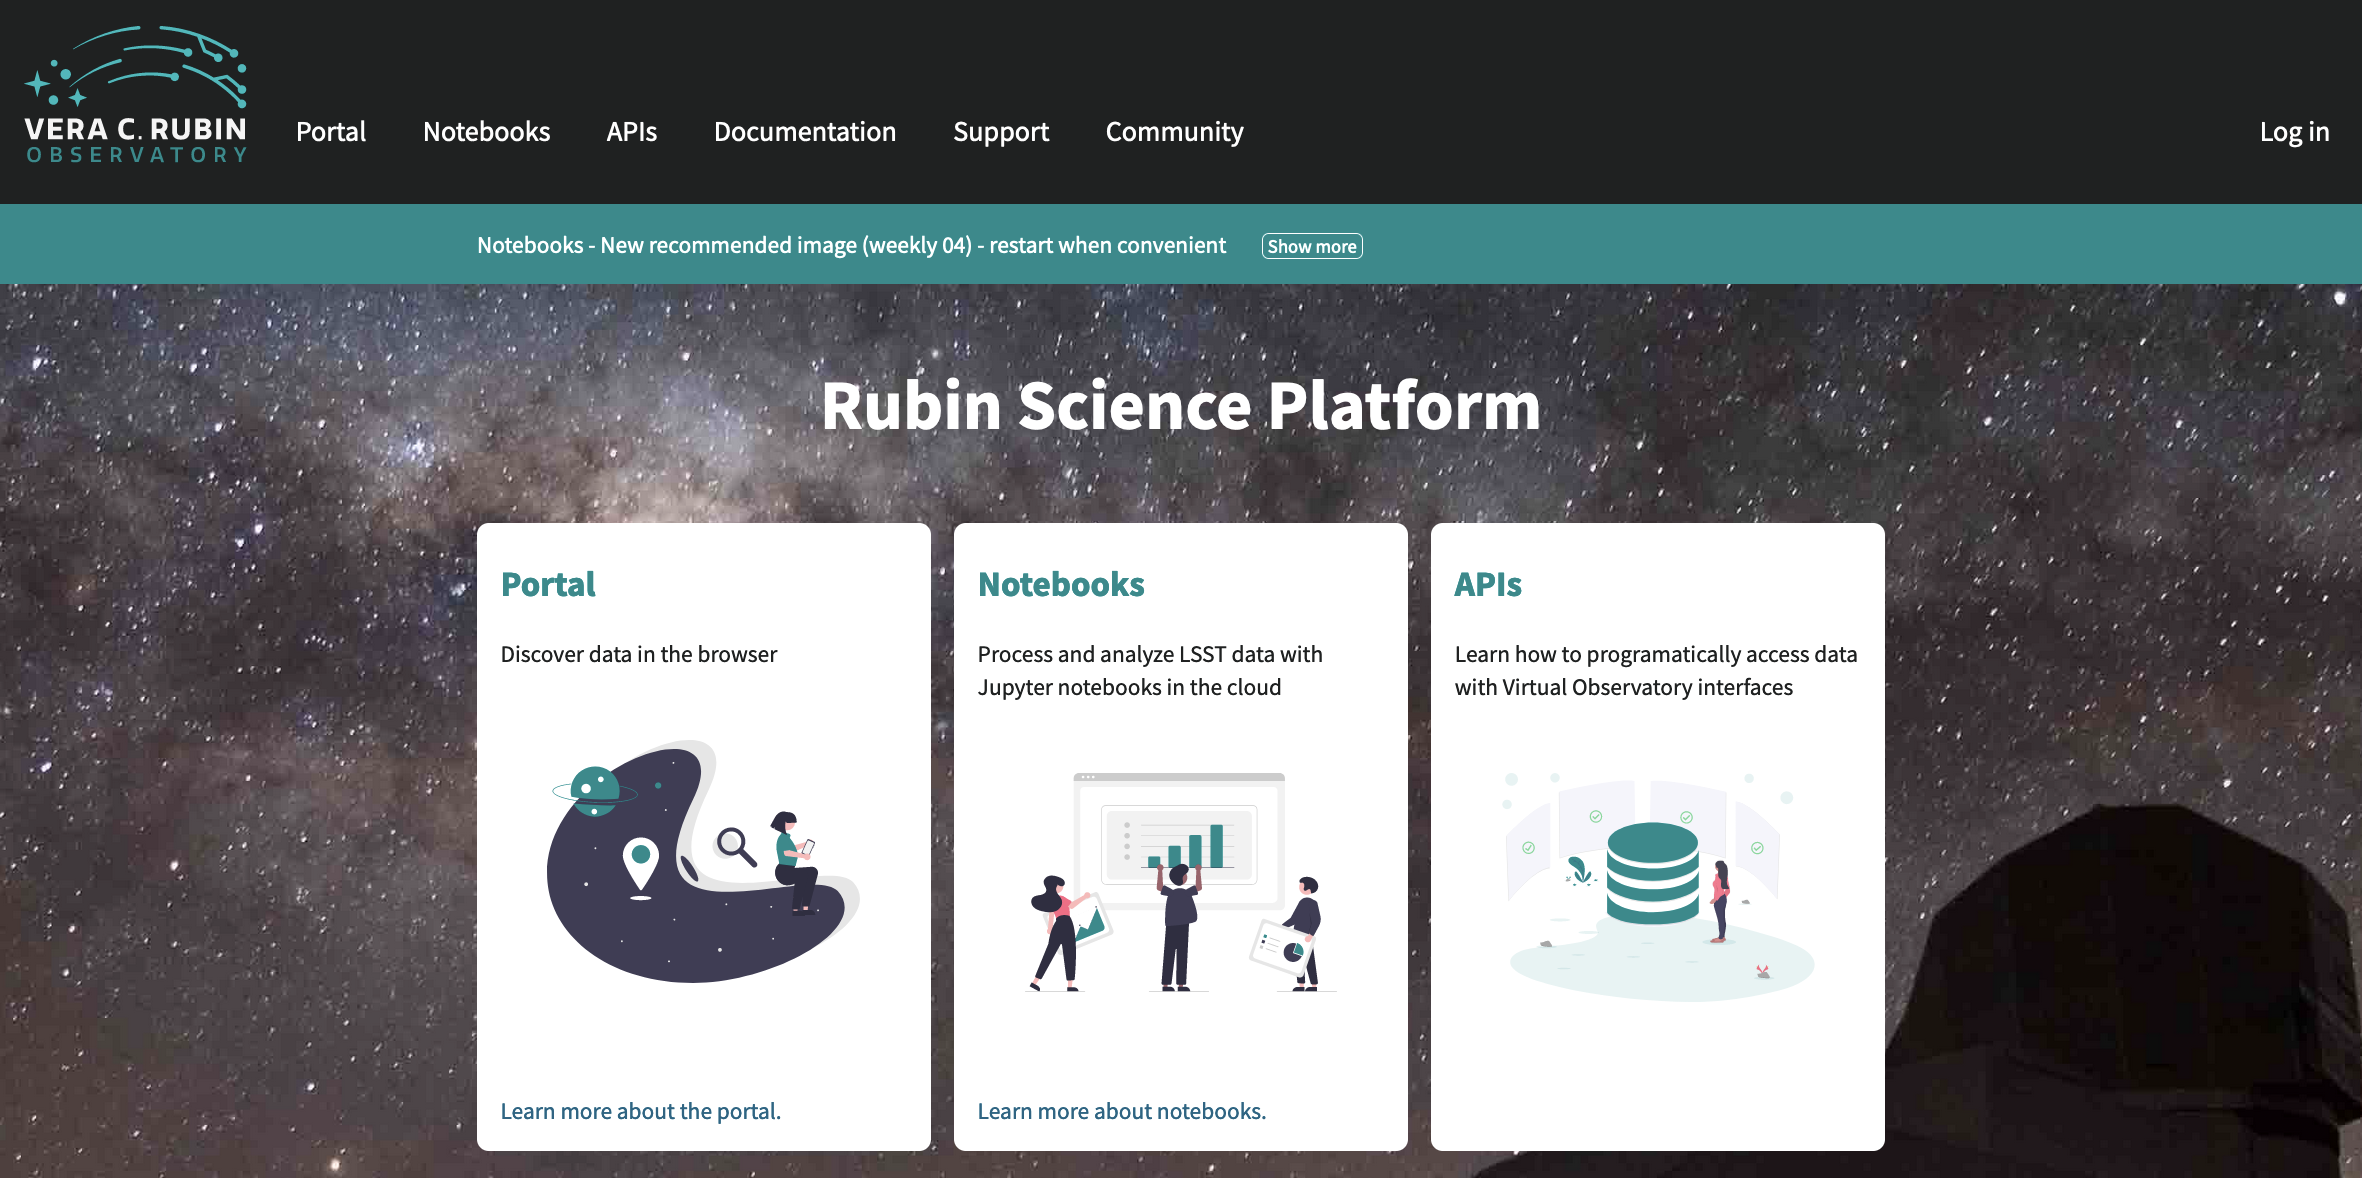
\includegraphics[width=0.9\textwidth]{RSP.png}
	\caption{ Users hosted on Google will typically use the Rubin Science Platform (RSP) depicted here.  \label{fig:goglearch}}
\end{centering}
\end{figure}


A requirement of this is the client server butler discussed  in this SPIE paper \cite{2024SPIE13101.129Jtmp}

\section {US Data Facility Architecture} \label{sec:usdfarch}


\begin{figure}
\begin{centering}
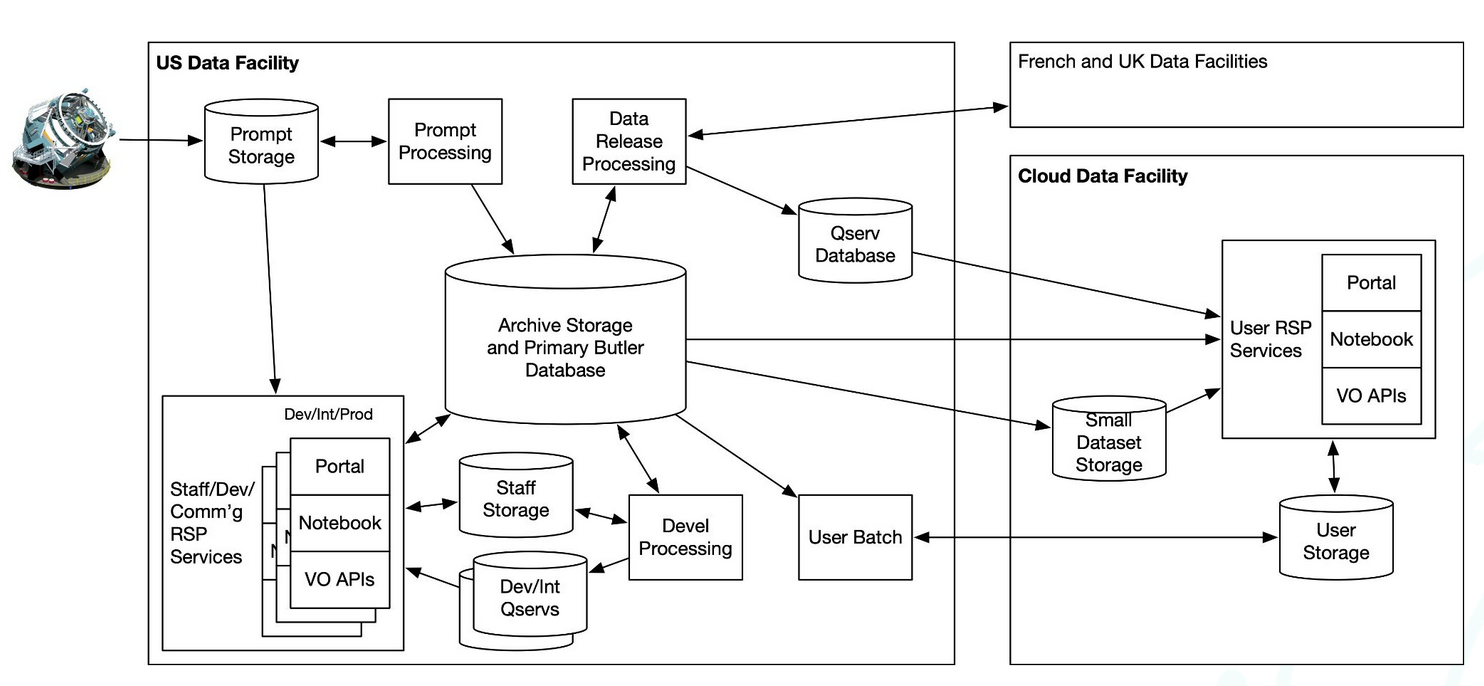
\includegraphics[width=0.9\textwidth]{hybrid}
	\caption{ Hybrid model: Data at SLAC but users on the cloud.  \label{fig:usdfarch}}
\end{centering}
\end{figure}

The scope for the USDF on-prem includes data production services:
prompt processing, serving alerts to the community and annual Data
Release Processing. The USDF acts as the archive for all data, and
provides the Qserv object catalog as well as access to image data, be
it cutouts or full images. It will provide batch cycles for cloud-based science users.
It will also act as a home for developers and staff (and
commissioners) to ensure data quality (see \autoref{fig:usdfarch}).


\subsection{Hardware}

The USDF is hosted by the SLAC Shared Scientific Data Facility
(S3DF) which is itself hosted in Stanford Research Computing Facility (SRCF).
SRCF accommodates projects from SLAC and Stanford, while the S3DF is the
focal system for SLAC projects. The USDF lives in a shared cluster and
benefits from economies of scale and standardization across S3DF
projects. It is also exposed to potentially disruptive activities by
other projects.

In order to support hundreds of PBs of storage, S3DF adopted the Weka
filesystem for high throughput. Weka is based on a tiered system with
Solid State Disks (SSD) backed by spinning disk. It presents a POSIX interface while the
backend is a Ceph object store. This system forms the basis of the
data archive. A tape robot provides storage for seldom-read data and
acts as a backup tier.

Batch processing is done on a Slurm cluster, currently primarily Advanced Micro Devices (AMD) milan
processors with 128 cores and 512 GB RAM per node.

Data is transported to the USDF from the summit over a combined
leased-line, ESNet-supported network with routing optimized via an
overlay. The leased line terminates in Atlanta, where ESNet takes
over. Traffic to the two other Data Facilities is also provided by
ESNet, connecting to the GEANT\footnote{pan-European data network for the research and education community}
 and Renater systems in Europe.

\subsection{Batch processing}

The USDF supports batch processing for a number of purposes: annual
multi-site data releases; pipelines teams testing for algorithms
performance; processing by individual developers for their algorithm
development; data quality checking and validation.

Multisite processing makes use of the Production ANd Distributed Analysis system (PanDA),\cite{2024CSBS....8....4M} developed
by ATLAS (A Toroidal LHC Apparatus) for the Large Hadron Colider (LHC).
It has a well-defined mechanism for routing work
from a central server to multiple remote locations. ATLAS has
demonstrated submitting millions of jobs per day to hundreds of sites.
A difference between typical astronomy and High Energy Physics (HEP) workflows is the
number of and duration of processes: astronomy tends to many more much
shorter jobs than HEP.\cite{2023arXiv231204921K} Significant effort was required working with the PanDA
team to cluster up short jobs to avoid prohibitive startup costs.
PanDA is a heavyweight solution to processing; local processing for
the pipelines teams and developers is done using HTCondor\footnote{\url{https://htcondor.org}}.

Data management and movement is also orchestrated by LHC tools: Rucio\footnote{\url{https://rucio.cern.ch}}
for data management and FTS3\footnote{\url{https://fts3-docs.web.cern.ch/fts3-docs/}} for movement. These tools also routinely
handle large numbers of files and transfers, however the difference between astronomy
and HEP persists here as well, with astronomy generating many more,
much smaller files than HEP. This will make the Rubin Rucio database
bigger than ATLAS's and will require some growth planning.

The large number of small files will also be a challenge for network
transfer. We are investigating zipping up large numbers of files both
for better transfer as well as easier storage on tape.

\subsection{Non-user-facing services}

Currently the primary reasons for putting services on-prem are a low
latency requirement for prompt processing, and the still-unfavorable
comparison of storage prices between on-prem and the cloud. To a lesser
degree, those comparisons also apply to CPU.

This means that Prompt Processing and Alerts production, with their
2-minute latency requirement are hosted on-prem. Additionally, there
are security requirements on data arriving at the USDF, including
physical measures implemented on the racks themselves.\cite{DMTN-199}

The large data volumes associated with the storage archive and Qserv
database hosted at the USDF implies that external access to them must be
provided by services.

Kubernetes is used to manage almost all our services, making use of
ArgoCD as well as our custom Phalanx system (see \S \ref{sec:deploy}).
Native Kubernetes tools
are used to manage standard services, such as Postgres databases,
making administration, backups, etc, scalable. Rucio and PanDA are
managed by Kubernetes to take advantage of these features.

The Prompt Processing framework executing the Alert Production is implemented
using Knative\footnote{\url{https://knative.dev/docs/}} on top of
Kubernetes to allow elastic instantiation, configuration, and teardown of
pods responding to notifications from the summit in advance of the
next visit.
Prompt Processing and Alert Distribution both use Kafka installed on Kubernetes.
We use the Strimzi Operator to install Kafka and for management.  Strimzi
has worked well to simplify installation, upgrades, and for maintaining
health of the Kafka clusters.

Three large database systems are minimally using Kubernetes, as they
are either commercial or custom services with no native Kubernetes
support. These are the Engineering and Facilities Database (EFD),\cite{2024SPIE13101.59Ftmp}
Qserv, and Cassandra systems, with Qserv the custom system.
The EFD is implemented with an InfluxDB Enterprise High Availability cluster.

For monitoring we use Prometheus\footnote{\url{https://prometheus.io}}.  Prometheus has native support for
Kubernetes metrics and many of the Kubernetes operators described earlier
like Strimzi and the Cloud Native Postgres (CNPG) natively provide metrics in Prometheus. We also
wrote some of our own metrics to track Prompt Processing.
We use Grafana for creating dashboards to visual metrics and for generating alarms when thresholds are crossed.
We use Loki from Grafana Labs to capture logs from Kubernetes pods
and from application level logs. Loki stores these logs in an on-premise S3 Ceph Cluster.

\section{Continuous Deployment across the Rubin facilities} \label{sec:deploy}

Early on we adopted Kubernetes which provided a service architectures that is well isolated from the underlying infrastructure.
This approach has already paid off massive dividends.
For example when funding lines suddenly shifted we were able to painlessly transition from an on-premises facility to an Interim Data Facility on Google Cloud.
Furthermore the Rubin Science Platform (RSP) became a generic data services platform that is currently deployed on eight distinct (and distinctly managed) infrastructures (on-prem and cloud).
Finally this has allowed us to leverage the Cloud for services like the RSP which benefit from its advantages such as elasticity, scalability, isolation.


\subsection{Division of responsibilities}
We have had ways to abstract system services from our developed services for some time, containers and java effectively allow one to run \emph{anywhere}.
These work well enough for single user single processor deployments.
When you need to scale up another level of orchestration is needed, kubernetes fits neatly between our infrastructure and our developed applications providing a powerful container orchestration and resource management system.

Our agreement with each facility is to provide a Kubernetes deployment platform upon which we may deploy our services.
It feels like the first time that this actually works well - we have to learned to make our applications portable of course but also the technology is so much better than any precursors.

Each thus provides a kubernetes environment with disk, network and compute resources upon which we spin up our services.
A vault for secrets is also needed.
From the service perspective each facility looks similar.

\subsection{Phalanx, Helm and ArgoCD}

Helm\footnote{https://helm.sh/} is a standard approach to tell Kubernetes about software.
For our purposes this is most usually a JSON file describing which github repo our code is in where the container is and how to start it.

Of course there are parts of this configuration which are site specific and parts which are generic.
For example the database URL for an application will be different in USDF and Summit, the \emph{value} of the database URL is different are each site, the URL variable is the same so the application does not change only the configuration.
Phalanx\footnote{phalanx.lsst.io} is our repository of configuration files for all of our deployments.
Within phalanx each application has a directory with a helm configuration - it also has a values file for each environment to specify the specific values for that environment.
Each environment also has a Vault configuration so that secrets such as database password may also be specified by an environment specific identifier.
Finally Phalanx has a list of deployed applications on each site.

Actually deployment is manged by ArgoCD\footnote{https://argo-cd.readthedocs.io/en/stable/}.
As the name implies ArgoCD provided continuous delivery for Kubernetes.
It interprets the configuration files stored in Phalanx to deploy containers on the kubernetes system associated with each environment.
This is a powerful system which can track the main or any given branch or tag of a github repository to keep the application in sync.

\subsection{Continuous Integration}
We rely on Github actions to build containers for each branch or tag of a given application


\section{Open Issues} \label{sec:open}

An open issue at this point is that we have not yet tested the client server butler between SLAC and Google.
We have checked the bandwidth and latency is acceptable but it remains to be seen how it will work under load.
~
~



\section{Conclusion} \label{sec:conc}
The Vera C. Rubin Observatory will come into operations in 2025.
The Rubin US data facility, hosted at SLAC, stores the Rubin data and processes it in conjunction with our French and UK partner facilities.

We have already run most of our scientist facing services on Google for three years.
We currently support one thousand users on the science platform hosted on Google and are preparing for the many thousands of more users Rubin expects.

Transition to a hybrid model with the bulk of the data stored on premises at SLAC but maintaining the scientist facing services on Google is underway.



\acknowledgments

This material is based upon work supported in part by the National Science Foundation through Cooperative Agreement AST-1258333 and Cooperative Support Agreement AST-1202910 managed by the Association of Universities for Research in Astronomy (AURA), and the Department of Energy under Contract No.\ DE-AC02-76SF00515 with the SLAC National Accelerator Laboratory managed by Stanford University.
Additional Rubin Observatory funding comes from private donations, grants to universities, and in-kind support from LSSTC Institutional Members.

\appendix
% Include all the relevant bib files.
% https://lsst-texmf.lsst.io/lsstdoc.html#bibliographies
%\section{References} \label{sec:bib}
\bibliographystyle{spiebib}
\bibliography{local,lsst,lsst-dm,refs_ads,refs,books}

% Make sure lsst-texmf/bin/generateAcronyms.py is in your path
\section{Acronyms} \label{sec:acronyms}
\input{acronyms.tex}

\end{document}
